%\documentclass[11pt,a4paper,openright]{report}
\documentclass[project,twoside]{iitbreport}

\usepackage[toc,page]{appendix}
\usepackage{titlesec}
\titlespacing\section{0pt}{12pt plus 4pt minus 2pt}{0pt plus 2pt minus 2pt}
\titlespacing\subsection{0pt}{12pt plus 4pt minus 2pt}{0pt plus 2pt minus 2pt}
\titlespacing\subsubsection{0pt}{12pt plus 4pt minus 2pt}{0pt plus 2pt minus 2pt}
%\titlespacing\subsection{0pt}{12pt plus 4pt minus 2pt}{0pt plus 2pt minus 2pt}

%% Selectively comment out sections that you want to be left out but
%% maintaining the page numbers and other \ref
%\includeonly{%
%  introduction,
%  ref,
%  conclusion
%}

%%% Some commonly used packages (make sure your LaTeX installation
%%% contains these packages, if not ask your senior to help installing
%%% the packages)
%\usepackage{pdfpages}
\usepackage{mathtools}
\usepackage{program}
\usepackage{algorithm}
\usepackage[noend]{algpseudocode}
\usepackage{booktabs}
\usepackage{fixltx2e}
\usepackage{url}
\usepackage{pbox}
\usepackage{graphicx}
\usepackage[T1]{fontenc}
\usepackage{enumitem}
\usepackage{amsmath}
%\usepackage{enumerate} %lower-case roman numerals in enumerate lists
\usepackage{multirow} %for table
\usepackage{hhline} %for table
\usepackage{subcaption} %for subcaption in sub-figures
\setlist{nosep}
\graphicspath{{images/}}
\newcommand{\dud}[1]{\underline{#1}}
%python
\usepackage{listings}
\usepackage{color}

\newcommand{\mle}{$ \le $}
\newcommand{\marr}{$ \rightarrow $}

\definecolor{codegreen}{rgb}{0,0.6,0}
\definecolor{codegray}{rgb}{0.5,0.5,0.5}
\definecolor{codepurple}{rgb}{0.58,0,0.82}
\definecolor{backcolour}{rgb}{0.95,0.95,0.92}

\lstdefinestyle{mystyle}{
	backgroundcolor=\color{backcolour},   
	commentstyle=\color{codegreen},
	keywordstyle=\color{magenta},
	numberstyle=\tiny\color{codegray},
	stringstyle=\color{codepurple},
	basicstyle=\footnotesize,
	breakatwhitespace=false,         
	breaklines=true,                 
	captionpos=b,                    
	keepspaces=true,                 
	numbers=left,                    
	numbersep=5pt,                  
	showspaces=false,                
	showstringspaces=false,
	showtabs=false,                  
	tabsize=2
}

\lstset{style=mystyle}
%python2 
% Default fixed font does not support bold face
\DeclareFixedFont{\ttb}{T1}{txtt}{bx}{n}{12} % for bold
\DeclareFixedFont{\ttm}{T1}{txtt}{m}{n}{12}  % for normal

% Custom colors
%\usepackage{color}
\definecolor{deepblue}{rgb}{0,0,0.5}
\definecolor{deepred}{rgb}{0.6,0,0}
\definecolor{deepgreen}{rgb}{0,0.5,0}

%\usepackage{listings}
% Python style for highlighting
\newcommand\pythonstyle{\lstset{
		language=Python,
		basicstyle=\ttm,
		otherkeywords={self,if,while,log},             % Add keywords here
		keywordstyle=\ttb\color{deepblue},
		emph={MyClass,__init__},          % Custom highlighting
		emphstyle=\ttb\color{deepred},    % Custom highlighting style
		stringstyle=\color{deepgreen},
		frame=tb,                         % Any extra options here
		showstringspaces=false            % 
	}}
%endpython
%\renewcommand{\chaptername}{}
\usepackage{titlesec}

\begin{document}
\title{Certification of Python Programs on the Basis of Static Information Flow Analysis}
\author{{\href{http://www.cse.iitb.ac.in/~kush/}{Abhishek Pratap Singh}}\\
	143050077\\
	\vspace{0.5cm} 
	\normalfont \textit{ \centerline{under the guidance of}}
	\vspace{1.0cm} 
	\newline
	{\textbf{Prof. R K Shyamsundar}}}
\degree{Master of Technology}
\dept{\href{http://www.cse.iitb.ac.in/}{Department of Computer Science and Engineering}}
\monthyear{July, 2016}

%\makecoverpage
\maketitle

\begin{abstract}
	In this thesis, we present our work on secure information flow analysis of python programs.
	We have built a platform that takes source code and labels of all objects used in python program as input for static
	analysis of information flow throughout the program. We started with Denning's lattice model [1]
	for verification of secure information flow. In this model, every object is associated with its
	security class. To prevent unauthorized leak of information, the flow of information should be
	in one way -- from less secure to more secure class. A lattice represents such information
	model very well, the upward direction in lattice represents secure information flow. Verification of
	information flow only on the basis of security class is not sufficient to certify the security of system, there is a need to consider the process, user or subject that executes the code. Use of Reader Writer Flow model \cite{denning} with subjects makes it possible to do secure
	information flow analysis. We have developed four type of constraint generators C1, C2, C3 and C4 each implementing different approach. Constraint generator C1 considers fixed label and PC reset(PC reset denotes PC is not retaining information out of scope), C2 considers fixed label and monotonic PC (monotonic PC never lose information), C3 considers dynamic label and PC reset and finally the constraint generator C4 considers dynamic label and monotonic PC. Constraint resolver takes these constraints and RWFM labels [2] for each
	object defined by the user as input and provides answers to various queries related to information
	flow security.The report describes, the approach, implementation and case study done so far.
\end{abstract}

\renewcommand{\abstractname}{\LARGE Acknowledgements}


%\clearpage
\pagenumbering{roman}
\addtocontents{toc}{\vskip-40pt}
\let\cleardoublepage\clearpage
\tableofcontents
\listoffigures
%\listoftables
\lstlistoflistings
\newpage
%\cleardoublepage
%\clearpage
\let\cleardoublepage\clearpage
\setcounter{page}{1}
\pagenumbering{arabic}

\chapter{Introduction}
\section{Language Based Security}
Information security is major concern nowadays. Systems are vulnerable to various attacks and exposed to threats via network. There are many approaches to enforce security policies in the system one of them is language based security, this approach focuses on enforcement of security policies on a application using program analysis. There are three main branches in language based security (a) Reference Monitor (b) Type Safe (c) Certifying Compiler this report focuses on certifying compiler, certifying compiler approach is based on program analysis compiler checks whether program follows security policy. Compiler does certification from outside of the system so it matches with principle of security model (i) Principle of least privilege (ii) Minimal computing base \cite{lang}. Static analysis is simple for this type of certification because whole process completes in a one go. Dynamic analysis becomes necessary if information flow occurs only at run time. So hybrid approach can cover all type of ananlysis.    
\section{Noninterference}
One of the earliest formal work in information security is concept of noninterference created by Goguen and Meseguer \cite{noni} in the context of MLS(Multi Level Secure). It gave concept to determine information leak in system of multiple users, suppose that there are two group of users A and B in a system S and if user of group A interacts with System S then view of users of B remains unchanged. This concept was developed for deterministic systems. Due to support for nondeterminism in most of programming languages, researcher \cite{ques} questioned relevance of noninterference for security of program. 
Volpano et al \cite{volpano} says that noninterference can be used for current day programming languages by using purely value based interpretation of noninterference, and with the help of Denning's certification semantics. Volpano's work regarding noninterference has set standards in language based security.          
\section{Security of a program}
There are various techniques to ensure security of program, information flow control is one of them. 

\subsection{Motivation}
In the field of data security, there are a lot of approaches to prevent leak of information for example cryptography takes care of confidentiality and integrity while data is transmitting through less secure networks, access permission on files prevent unauthorized access to files in a system where users have different privileges. But at the time of execution of program, data used in the program is vulnerable to various attacks so to maintain security at the time of execution of program and processing of data, information flow policies are used. The subject is defined as an executing authority it can be a user or parent process, object can be a file, program variable, memory location etc. In a multilevel security system a subject has permission related to objects. Information flow verification of program only considering objects may seem to be secure but with a particular subject same program may be insecure, so we considered subjects in static analysis of python program.   

\subsection{Goals}
To develop a platform that takes input a python program and labels of each variable used in the program, and provide answers to various queries regarding the security of information flow.   

\chapter{Related work}
\label{ch:related}
There have been many studies on information flow control and all of them share some basic properties like information flow should be from less secure entity to more secure entity. Denning's book \cite{denning} has a chapter on information flow control, this chapter describes lattice model for information flow \cite{lattice}, this makes it easy to track information flow in a program using transitivity property. Analysis has been done on basic operations which involve information flow like assignment operation (explicit flow) based on data flow, conditional operations like if else, while etc. (implicit flows) based on control flow, information flow through covert channel based on traps and exception in programs. Here are some basic rules given in \cite{denning}, (arrow $\rightarrow$ denotes information flow).  
\begin{itemize}
	\item x = y : y $\rightarrow$ x
	\item if e then x = y : e $\rightarrow$ x
	\item while w {if e then{ x = y} w =false } : w $\oplus$ e $\rightarrow$ x
	\item infinite loop: while w {}; x = y :- w $\rightarrow$ x etc.   
\end{itemize}
Chen et al. \cite{hybrid}(published in 2014) presented work on python byte-code and claimed that there was no work related to python at that time. They implemented information flow checker for python byte-code using static and dynamic analysis but their main focus is on information flow policies related to objects. Kumar et al. \cite{rwfm} introduce a new model to work with subjects and my work will be focused on this. Conti et al. \cite{taint} provide library support in python for information flow analysis in explicit flows only.       
  

\chapter{Information Flow Analysis using Denning's Lattice Model}
\label{ch:denning}
\section{Analysis In Local Scope}
We started certification of python code at local scope initially.
\begin{figure}[ht]
	
	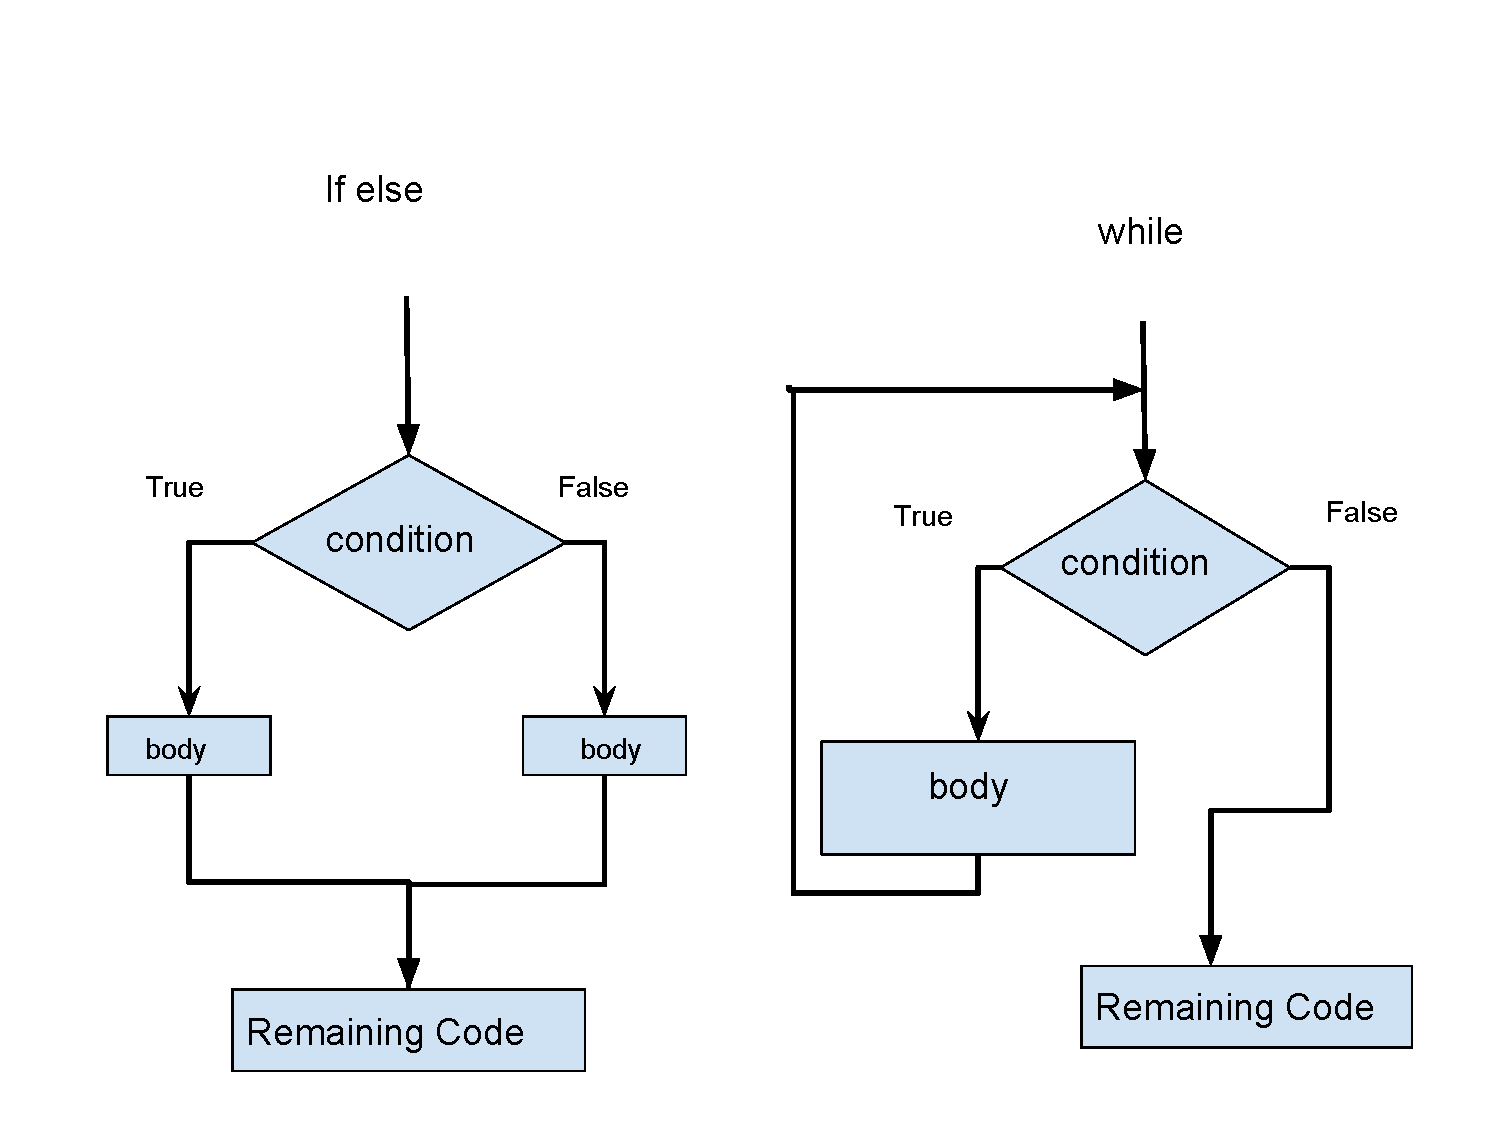
\includegraphics[width=0.8\textwidth]{branching}
	\caption{Control flow graph of If else and while loop}
	\label{fig:branching}
\end{figure}
In figure \ref{fig:branching} we considered information flowing from variables used in condition to targets of assignment operation in body code only. Further analysis will be dealing with information flows to targets of assignment in remaining code. Now a program with if else and terminating loops can be certified to be secure (no information leaks) by using basic rules of information theory implemented in my script.\\
\textit{Fifth chapter of Denning's book\cite{denning} used six examples to describe how can information flow through different ways in the program. We used python version of these examples as benchmark.}\\
\subsection{Benchmarking of Certification Script using Denning's Examples \cite{denning}}
\begin{lstlisting}[language=Python, caption=Python version of copy1 example in \cite{denning}. goal: information flow from x to y, label={lst:copy1} ]
#Procedure copy1
x = 0
z = 0
y = 0
if x == 0:
	z=1
if z == 0:
	y=1
\end{lstlisting}
Constraints for program in \ref{lst:copy1} generated by our script are:\\
\begin{enumerate}
	\item low $\leqslant$ \dud{x}
	\item low $\leqslant$ \dud{z}
	\item low $\leqslant$ \dud{y}
	\item low $\leqslant$ \dud{y}
	\item \dud{x} $\leqslant$ \dud{z}
	\item \dud{z} $\leqslant$ \dud{y}
\end{enumerate}
Program in listing \ref{lst:copy1} shows how  information can flow indirectly from x to y, for secure information flow $ \dud{x} \leqslant \dud{y} $ must be true. Constraint 5 (x $\leqslant$ z) and constraint 6 (z $\leqslant$ y) with transitivity property of lattice model satisfies x $\leqslant$ y.  \\
\begin{lstlisting}[language=Python, caption=Python version of copy2 example in \cite{denning}. goal: information flow from x to y, label={lst:copy2} ]
# Procedure copy2
x = 0
z = 1
y = -1
while z == 1:
	y = y + 1
	if y == 0:
		z = x
	else:
		z = 0
\end{lstlisting}
Constraints of program in Listing \ref{lst:copy2} generated by our script are:\\
\begin{enumerate}
\item low $\leqslant$ \dud{x}
\item low $\leqslant$ \dud{z}
\item low $\leqslant$ \dud{y}
\item \dud{y} $\oplus$ \dud{z} $\leqslant$ \dud{y}
\item \dud{y} $\oplus$ \dud{x} $\oplus$ \dud{z} $\leqslant$ \dud{z}	
\end{enumerate}
Information flows from x to y using iteration of the while loop in listing \ref{lst:copy2}.
One iteration of while loop changes the value of y to -1 to 0 by incrementing it by 1, and two iteration of same while loop changes the value of y to -1 to 1. Number of iterations of while loop depends on value of x so this program is transmitting information from x to y indirectly using both explicit and implicit information flows.\\  
\textbf{\textit{Proof:}}\\
\dud{x} $\leqslant$ \dud{y} must be true for secure information flow. This can be proved using constraint 4 ( \dud{y} $\oplus$ \dud{z} $\leqslant$ \dud{y})
and constraint 5 (\dud{y} $\oplus$ \dud{x} $\oplus$ \dud{z} $\leqslant$ \dud{z}) in two ways. First: \dud{z} $\leqslant$ \dud{y} is given in constraint 4 and \dud{y} $\leqslant$ \dud{z} is given in constraint 5 so \dud{y} must be equal to \dud{z} using this new constraint ( \dud{y} $\equiv$ \dud{z} ) and reduced constraint 5 (\dud{x} $\leqslant$ \dud{z}) desired constraint \dud{x} $\leqslant$ \dud{y} is proved.  
\section{Further analysis: considering global influence of while}
A program either terminates after a finite period of time or executes for an infinite period of time. The latter can be achieved through while loop and for loop. Such a non-terminating loop influences variables within the body of the loop as well as after the body of loop.
 \begin{lstlisting}[language=Python, caption=Non terminating while., label={lst:ntwhile} ]
 x = 0
 z = True
 y = 0
 while z :
	 y = 5
x = 5	
 \end{lstlisting}
In listing \ref{lst:ntwhile} execution of last statement x = 5 is conditioned on "while z" statement similar to "if" branching but "if" has limited body but in this case every statement that comes after "while z" share fate with x = 5, because of this property of "while" it is very crucial to know whether loop is terminating or nonterminating, so either there should be a mechanism to determine to terminating and nonterminating nature of loop or treat all while loop as nonterminating, latter approach is imprecise but secure, for now we are using this approach to handle while loops.
\subsection{Benchmarking of Certification Script using Denning's Examples \cite{denning}}
\begin{lstlisting}[language=Python, caption=Python version of copy5 example in \cite{denning}. goal: information flow from x to y, label={lst:copy5} ]
#Procedure copy5
y = 0
while x==0 :
	pass
y = 1
\end{lstlisting}  
Constraints generated by our script:
\begin{enumerate}
	\item low $\leqslant$ \dud{y}
	\item \dud{x} $\leqslant$ \dud{y}
\end{enumerate}
so here our script able to track information flow from x to y and generating constraint \dud{x} $\leqslant$ \dud{y} for verification.

\begin{lstlisting}[language=Python, caption=Python version of copy4 example in \cite{denning}. goal: information flow from x to y, label={lst:copy4} ]
#Procedure copy4
import thread
import time
import threading

def thread1():
global x
global e0
global e1
if x==0:
	e0 = False
else:
	e1 = False

def thread2(): 
global e0
global e1
global y
while e0
	pass
y = 1
e1 = False

def thread3():
global e1
global e0
global y
while e1:
	pass
y = 0
e0 = False

thread.start_new_thread(thread1,())
thread.start_new_thread(thread2,())
thread.start_new_thread(thread3,())\end{lstlisting}

Constraints generated by our script for program in listing \ref{lst:copy4} are:
\begin{enumerate}
	\item \dud{x} $\leqslant$ \dud{e0}
	\item \dud{x} $\leqslant$ \dud{e1}
	\item \dud{e0} $\leqslant$ \dud{y}
	\item \dud{e0} $\leqslant$ \dud{e1}
	\item \dud{e1} $\leqslant$ \dud{y}
	\item \dud{e1} $\leqslant$ \dud{e0}
\end{enumerate}
(\dud{x} $\leqslant$ \dud{e0} ) and (\dud{e0} $\leqslant$ \dud{y}) \hspace{1cm} $\equiv$ \hspace{1cm} \dud{x} $\leqslant$ \dud{y} (transitivity)\\
(\dud{x} $\leqslant$ \dud{e1} ) and (\dud{e1} $\leqslant$ \dud{y}) \hspace{1cm} $\equiv$ \hspace{1cm} \dud{x} $\leqslant$ \dud{y}\\
So script able to track hidden information flow from x to y and generating constraint for this flow \dud{x} $\leqslant$ \dud{y} by using transitivity.

\chapter{Analysis of Multi-threaded Programs}
\label{ch:thread}
In a multi-threaded program, information flows among threads because of communication and synchronization among them. There are two types of semaphores --- counting and binary, for synchronization among threads. For now, our script handles binary semaphores only. 
\section{Handling Information flow due to WAIT and SIGNAL operations}
Traditional operations related to binary semaphore are WAIT and SIGNAL. SIGNAL operation changes the value of semaphore 0 to 1 and WAIT operation wait for an infinite time if the current value of the semaphore is 0 otherwise it changes value 1 to 0 and allows control flow forward. There are three operations related to the binary semaphore in python language wait(), set() and clear(). Traditional WAIT operation can be simulated using python wait() followed by clear() operation, SIGNAL is equivalent to set().\\~\\
\begin{minipage}[b]{0.45\linewidth}
	\centering
	\begin{lstlisting}[ numbers=left, mathescape,%
	caption={Example of wait() operation on binary semaphore.Info Flow: s$\rightarrow$x}, label=lst:wait]
	s = threading.Event()
	s.wait()
	x = 1
	
	\end{lstlisting}
\end{minipage}
\hspace{0.5cm}
\begin{minipage}[b]{0.45\linewidth}
	\centering
	\begin{lstlisting}[ mathescape,%
	caption={Infinite while loop, Information Flow: x$\rightarrow$y }, label=lst:whilewait]
	y = 0
	while x:
		pass
	y = 1
	\end{lstlisting}
\end{minipage}\\
Listing \ref{lst:wait} and Listing \ref{lst:whilewait} show that control flow of wait()  is similar to infinite while loop so we treat wait() in a similar way. All statements which use global variables as a target of assignment and are preceded by wait() may transmit information to other threads. So information flows from semaphore $s_0$ to targets of assignment operations which follows $s_0$.wait() statement.\\
All semaphore operations simplified into normal operations.
\begin{itemize}
	\item s.set() treated as \textbf{s = s + 1}.
	\item s.clear() treated as \textbf{s = s - 1}.
	\item Listing \ref{lst:wait} and \ref{lst:whilewait} shows s.wait() equivalent to \textbf{while(s == 0) \{ skip \}}.
\end{itemize}
\subsection{Benchmarking of Certification Script using Denning's Example \cite{denning}}
\begin{lstlisting}[language=Python, caption=Python version of copy3 example in \cite{denning}. goal: information flow from x to y, label={lst:copy3} ]
#Procedure copy3
import thread
import time
import threading
s0 = threading.Event()
s1 = threading.Event()

def thread1():
	global x
	if x==0:
		s0.set()
	else:
		s1.set()

def thread2():
	global y
	s0.wait()
	s0.clear()
	y=1
	s1.set()

def thread3():
	global y
	s1.wait()
	s1.clear()
	y=0
	s0.set()

thread.start_new_thread(thread1,())
thread.start_new_thread(thread2,())
thread.start_new_thread(thread3,())
\end{lstlisting}

To certify the multi-threaded program in Listing \ref{lst:copy3} correctly our script must track information flow from x to y (x $\rightarrow$ y) and must generate constraints accordingly.\\
Constraints generated by our script for program in Listing \ref{lst:copy3} are:
\begin{enumerate}
	\item \dud{x} $\oplus$ \dud{s0} $\leqslant$  \dud{s0}
	\item\dud{x} $\oplus$ \dud{s1} $\leqslant$  \dud{s1}
	\item\dud{s0} $\leqslant$ \dud{s0}
	\item\dud{s0} $\leqslant$ \dud{y}
	\item\dud{s1} $\oplus$ \dud{s0} $\leqslant$  \dud{s1}
	\item\dud{s1} $\leqslant$ \dud{s1}
	\item\dud{s1} $\leqslant$ \dud{y}
	\item\dud{s1} $\oplus$ \dud{s0} $\leqslant$  \dud{s0}
\end{enumerate}  
constraint 1 (\dud{x} $\oplus$ \dud{s0} $\leqslant$  \dud{s0}) and constraint 4 (\dud{s0} $\leqslant$ \dud{y}) \hspace{1cm} $\equiv$ \hspace{1cm} \dud{x} $\leqslant$ \dud{y}.\\
constraint 2 ( \dud{x} $\oplus$ \dud{s1}    $\leqslant$  \dud{s1}) and constraint 7 ( \dud{s1} $\leqslant$ \dud{y}) \hspace{1cm} $\equiv$ \hspace{1cm} 
\dud{x} $\leqslant$ \dud{y}.\\	
Hence script is able to generate correct constraints in multi-threaded program too.
      

\chapter{ Category 1 constraint Generator : PC reset and fixed labels.}
\label{ch:c1}
This chapter describes working of first algorithm for constraint generation. All four algorithms are different because of different combination of PC label management scheme and  use of dynamic labels. In this algorithm we are using fixed label. Fixed label denotes that label will not change throughout the program. PC reset denotes that after completion of scope of a particular conditional/iteration body PC reset back to the PC just before the execution of conditional/iteration statement. PC monotonic denotes a scheme in which PC label never lose any information once it acquires, it just grows monotonically. This algorithm is able to capture basic information flows within a program, so this algorithm will certify a large number of programs as secure. Program certified secure by this algorithm does not mean that its fully secure, it certifies secure because of the limitation in detection of information flows in program. Some information flows which are not captured by this algorithm may violate information security.\\
\section{Working}
All four algorithm shares same basic structure for parsing input program. Dynamic analysis can not process all branches in a one go but static analysis process all branches in one run. Algorithms generates constraints for all possible control branches in program.  PC keeps track of variables used in conditional statement and iteration statement. Assignment operation are responsible for information flows so at each occurrence of assignment operation constraints generated with the help of PC label.
\section{Constraint Rules}
\begin{enumerate}
	\item < x := e > generate constraint [$\lambda(e)\oplus\lambda(PC)\le\lambda(x)$] and update PC label\\ $\lambda(PC) = \lambda(e)\oplus\lambda(PC)$ 
	\item < x := e > generate constraint [$\lambda(e)\oplus\lambda(PC)\le\lambda(x)$] and update PC label\\ $\lambda(PC) = \lambda(e)\oplus\lambda(PC)$ 
	\item < if e then c1 else c2>  $\forall  x \in ( modified\_global(\hspace{0.2cm} c1 \hspace{0.2cm}and \hspace{0.2cm} c2) \cup \{PC\} )$ generate constraints [$\lambda(e)\oplus\lambda(PC)\le\lambda(x)$] and update PC label $\lambda(PC) = \lambda(e)\oplus\lambda(PC)$
		
	\item < while e do c > $\forall  x \in ( modified\_global(c) \cup \{PC\} )$ generate constraints [$\lambda(e)\oplus\lambda(PC)\le\lambda(x)$] and update PC label $\lambda(PC) = \lambda(e)\oplus\lambda(PC)$
\end{enumerate}

\begin{figure}
	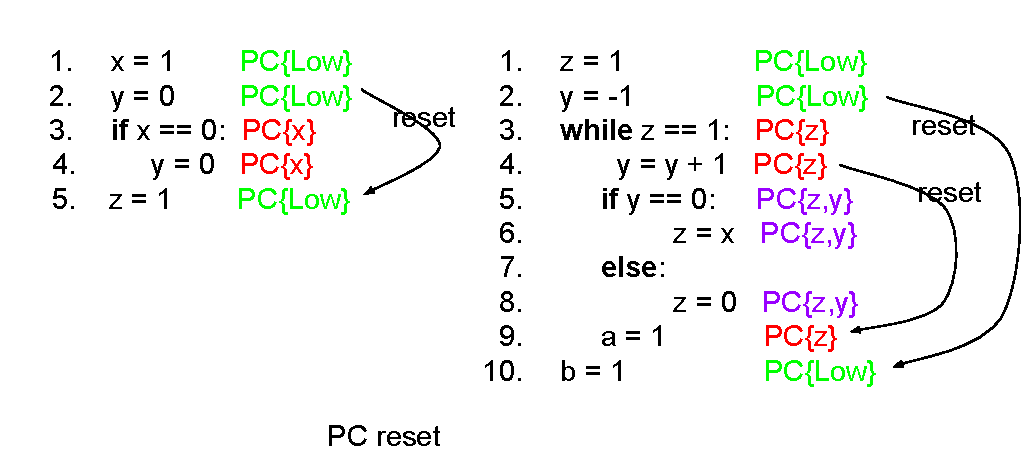
\includegraphics[width=1\textwidth]{PC_reset.pdf}
	\centering
	\caption{Example for PC reset}
	\label{fig:pcreset}
\end{figure}
\begin{figure}
	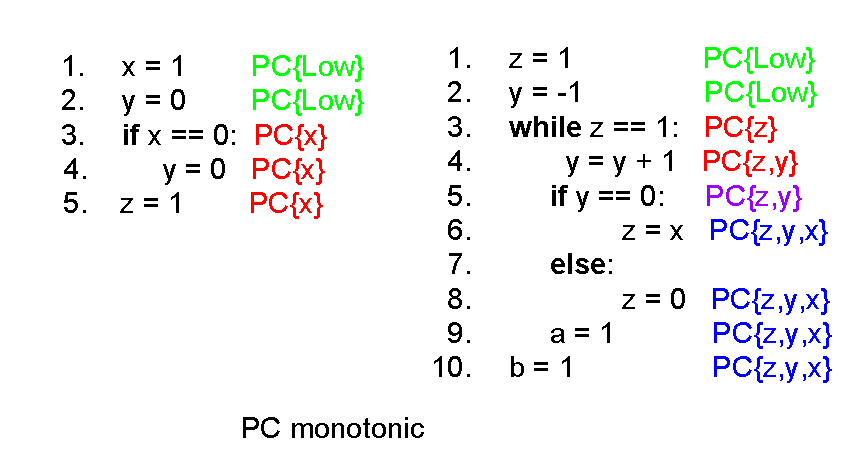
\includegraphics[width=1\textwidth]{PC_monotonic.pdf}
	\centering
	\caption{Example for PC monotonic}
	\label{fig:pcreset}
\end{figure}
\section{Key Idea}
Direct information flow happens because of copying or assigning values. Implicit information flow happens because of control dependency, this algorithm focuses on information flow from variables used in condition statement of if else(conditional)
and while(iteration) to all variables modified in the body of iteration or conditional.
\begin{lstlisting}[language=Python,caption={Python example}, label={lst:p1copy1}]
def(x,y):     #copy x to y
y = 0
z = 0
if x == 0:    # implicit flow x -> z PC{x}
	z = 1
if z == 0:    # implicit flow z-> y PC{z}
	y = 1
p = q         # direct flow q -> p PC{q}
\end{lstlisting}
Constraints generated by this algorithm for listing \ref{lst:p1copy1} are given below. 
\begin{itemize}
	\item x <= z
	\item z <= y
\end{itemize}
\section{Limitations}
For listing \ref{lst:p1copy1} this algorithm is able to capture all information flows, but in more complex programs it may declare falsely a program secure.
\begin{lstlisting}[language=Python, caption=Python version of copy5 example in \cite{denning}. goal: information flow from x to y, label={lst:p1copy5} ]
#Procedure copy5
y = 0
while x==0 :
pass
y = 1
\end{lstlisting}
For listing \ref{lst:p1copy5} this algorithm generated only one constraint Low <= y, that shows this algorithm will certify listing \ref{lst:p1copy5} secure always irrespective of information flow x to y is secure or not. All these limitation in capturing information flow raised because of PC label management in this algorithm is only focus on local information flow. Next algorithm will try to remove these limitation using monotonic PC label management. Appendix A shows the implementation of this algorithm.
\begin{lstlisting}[language=Python, caption=Python version of dynamic label example in \cite{denning}. goal: information flow from x to y, label={lst:p1dynamic} ]
def fun(x, y, z):
a = x
y = a
a = z
fun(x, y, z)
\end{lstlisting}
Another limitation of this algorithm is related to use of fixed label. In listing \ref{lst:p1dynamic} this algorithm detect false information flow z to y. Category 3 uses both dynamic and fixed label to remove this limitation. 
\chapter{Category 2 constraints : PC monotonic and fixed labels.}
This chapter describes working of category 2 constraint generator. This algorithm is a improved version of previous category 1 algorithm. This algorithm using monotonic PC label instead of PC reset. By using monotonic PC this algorithm is able to detect additional information flows in program.
\section{Working}
rules
\section{Key Idea}
This analysis extension of previous algorithm, non terminating loops
create a control dependency between variables used in condition of loop and
the rest of the code where control can go subsequently on termination of loop,
because of this behavior of non terminating loop PC storing all the dependencies.

\section{Limitations}  
In static analysis if constraint resolver ignores the order of generated constraints then it may show some additional false information flow in program, this is responsible for overhead and imprecision in certification process. Use of dynamic label solves this problem easily on the cost of more complex analysis.
\begin{lstlisting}[language=Python, caption=Python version of dynamic label example in \cite{denning}. goal: information flow from x to y, label={lst:p2dynamic} ]
def fun(x, y, z):
a = x
y = a
a = z
fun(x, y, z)
\end{lstlisting}
constraints generated for listing \ref{lst:p2dynamic} are given below:
\begin{itemize}
	\item x <= a
	\item a + x <= y
    \item a + x + z <= a
\end{itemize}
these constraints shows that there is information flow z to y ( using a <= y and z <= a) but in program there is no such flow exist. Because of such information flow constraint resolver may certify a secure program as not secure and it also create extra overhead on resolver. This example shows flaw in approach of using fixed label everywhere. Next algorithm will try to remove this limitation.



\chapter{Category 3 constraints : PC reset and dynamic labels.}
\label{ch:c3}
This chapter describes category 3 constraint generator. This algorithm introduces use of dynamic label. Global variable are using fixed label and all local variables are assigned dynamic label. Information can flow outside only because of modification of global variable, modification of local variable doe not cause information because information remains in program itself.   
\section{Constraint Rules}
\begin{itemize}
	\item < x := e > generate constraint [$\lambda(e)\oplus\lambda(PC)\le\lambda(x)$] and update PC label\\ $\lambda(PC) = \lambda(e)\oplus\lambda(PC)$ 
	\item < if e then c1 else c2> \begin{enumerate}
		\item $\forall  x \in ( modified\_global(\hspace{0.2cm} c1 \hspace{0.2cm}and \hspace{0.2cm} c2) \cup \{PC\} )$ generate constraints [$\lambda(e)\oplus\lambda(PC)\le\lambda(x)$] and update PC label $\lambda(PC) = \lambda(e)\oplus\lambda(PC)$
		\item $\forall x \in ( modified\_local(\hspace{0.2cm} c1 \hspace{0.2cm}and \hspace{0.2cm} c2) \cup \{PC\} )$ update PC label $\lambda(PC) = \lambda(e)\oplus\lambda(PC)$
	\end{enumerate}
	\item < while e do c > \begin{enumerate}
		\item $\forall  x \in ( modified\_global(c) \cup \{PC\} )$ generate constraints [$\lambda(e)\oplus\lambda(PC)\le\lambda(x)$] and update PC label $\lambda(PC) = \lambda(e)\oplus\lambda(PC)$
		\item $\forall x \in ( modified\_local(c) \cup \{PC\} )$ update PC label $\lambda(PC) = \lambda(e)\oplus\lambda(PC)$
	\end{enumerate}
\end{itemize} 
In static analysis if constraint resolver ignores the order of generated constraints then it may show some additional false information flow in program, this is responsible for overhead and imprecision in certification process.
Use of dynamic label solves this problem easily on the cost of more complex analysis.\\~\\
'a' is a local variable in function defined below.\\
def function(x,y,z):\\
\hspace*{1cm}a = x\\
\hspace*{1cm}y = a\\
\hspace*{1cm}a = z\\~\\
static analysis will generate constraints 1. x$\le$a, 2. a$\le$y, 3. z$\le$a.\\
Last two constraints shows false information flow from z to y (z\marr y).\\~\\
Dynamic label analysis\\
1. $\lambda(a)$ := x\\
2. $y\le \lambda(a) \{x\}$\\
3. $\lambda(a) := z $\\~\\
This analysis treats global and local variable differently so it avoids false constraints successfully without tracking order of constraints explicitly.\\~\\
a = x\\
while 1:\\
\hspace*{1cm} y = a\\
\hspace*{1cm} a = z\\~\\
Dynamic label Analysis:\\
First iteration of while:\\
1. $\lambda(a)$ := x\\
2. $y\le \lambda(a) \{x\}$\\
3. $\lambda(a) := z $\\~\\
Second Iteration:\\
2. $y\le \lambda(a) \{z\}$\\
3. $\lambda(a) := z $\\~\\
Dynamic label analysis generating different constraints for first iteration and second iteration but static analysis is not able to distinguish between information flow in first iteration and second iteration of while loop.
\section{Key Idea}
Definition of information flow among objects : If any data can be
guessed by using given objects which was unknown previously, by using this
idea information can flow outside only because of modification of global objects,
so any information flow from local objects to global objects must be
checked for security breach. Local variable plays a role of temporary in flow
of information from one global to another, so local variable must keep track
of information they hold, dynamic label is a good technique to keep track of
history of information stored in a local variable.
\section{Limitations}
This constraint generator again using PC reset label scheme. We created this category for thorough analysis and comparison among all categories. So it shares the first limitation of category 1. It fails to capture global information flows created by non terminating loops.   

\chapter{Category 4 constraints: PC monotonic and dynamic label.}
\label{ch:c4}
This algorithm is best among all four algorithm in terms information security. Dynamic label processing increases time complexity of this algorithm but we used a property of PC label to make optimization.
Constraint generation rules are same as category 3.
\section{Key Idea} In this analysis PC never gets reset because we want to track all possible information flows including information flows from a nonterminating loop to rest of code.\\ 
'a' is a local var\\
a = x\\
while w:\\
\hspace*{1cm} y = a\\
\hspace*{1cm} a = z\\
z = y\\~\\
Dynamic label Analysis:\\
1. $\lambda(a) = x$\\
2.PC\{w\}\\
3.PC\{w, $\lambda$(a)\{x\}\} \hspace{1cm} $w\oplus x \le y$\\
4.$\lambda(a) = z$\\
5.PC\{w, x, y\} \hspace{1cm} $w\oplus x\oplus y \le z$\\

So this algorithm is capable to track information flow w\marr z in last statement z = y by using monotonic PC without generating additional false constraints. 
\section{Limitations}
Use of dynamic label with monotonic creates challenge for processing of large number of labels.  

\chapter{Comparison among all categories of constraints.}
\label{ch:comp}
\begin{table}
\hspace{-2cm}
\begin{tabular}{|l|l|l|l|l|}
	\hline
	Input Program  &  C1 & C2 & C3 & C4 \\
	\hline
\begin{lstlisting}[language=Python]
#'a' is a local var
a = x
while w:
	y = a
	a = z
z = y
\end{lstlisting}&
\begin{lstlisting}
x <= a
a + w <= y
z + w <= a
y <= z
\end{lstlisting}&
\begin{lstlisting}
x <= a
a + x + w <= y
a + x + z + w <= a
a + x + z + w <= y
a + x + z + y + w <= z
y + x + w <= z
\end{lstlisting}&
\begin{lstlisting}
x + w <= y
x + z + w <= y
y <= z	
\end{lstlisting}&
\begin{lstlisting}
x + w <= y
x + z + w <= y
y + x + w <= z
y + x + z + w <= z	
\end{lstlisting}\\
	\hline
	
\end{tabular}
\caption{Example for comparison}
\label{tbl:compex}
\end{table}


Example given in table \ref{tbl:compex} is suitable to differentiate between all category.
First algorithm fails to track information flow w\marr z in last statement z = y.
Second algorithm is able to track information flow w\marr z in last statement z = y but it will show additional false information flow z \marr y too. 
Third algorithm avoids tracking of additional false information flow z \marr y but it fails to show information flow w \marr z because of PC reset.
Fourth analysis avoids tracking of false information flow as well as tracks information flow caused by nonterminating loop( w \marr z). Table \ref{tbl:compcopy} shows constraints generated for copy program given in Denning,s book by all constraint generator.
\begin{table}
\hspace{-2cm}
\begin{tabular}{|l|l|l|l|l|}
	\hline
	Programs  &  C1 & C2 & C3 & C4 \\
	\hline
	Copy1&
	\begin{lstlisting}
	x <= z
	z <= y
	\end{lstlisting}&
	\begin{lstlisting}
	x <= z
	x + z <= y
	\end{lstlisting}&
	\begin{lstlisting}
	x <= y
	\end{lstlisting}&
	\begin{lstlisting}
	x <= y
	\end{lstlisting}\\
	\hline
	Copy2&
	\begin{lstlisting}
	Low <= z
	Low <= y
	y + z <= y
	y + x + z <= z
	y + z <= z
	\end{lstlisting}&
	\begin{lstlisting}
	Low <= z
	Low <= y
	y + z <= y
	y + x + z <= z
	y + z <= z
	y + x + z <= y
	\end{lstlisting}&
	\begin{lstlisting}
	Low <= y
	y <= y
	y + x <= y
	\end{lstlisting}&
	\begin{lstlisting}
	Low <= y
	y <= y
	y + x <= y
	\end{lstlisting}
	\\
	\hline
	Copy3&
	\begin{lstlisting}
	x + s0 <= s0
	x + s1 <= s1
	s0 <= s0
	Low <= y
	s1 <= s1
	\end{lstlisting}&
	\begin{lstlisting}
	x + s0 <= s0
	x + s1 <= s1
	s0 <= s0
	s0 <= y
	s1 + s0 <= s1
	s1 <= s1
	s1 <= y
	s1 + s0 <= s0
	\end{lstlisting}&
	\begin{lstlisting}
	x + s0 <= s0
	x + s1 <= s1
	s0 <= s0
	Low <= y
	s1 <= s1
	\end{lstlisting}&
	\begin{lstlisting}
	x + s0 <= s0
	x + s1 <= s1
	s0 <= s0
	s0 <= y
	s1 + s0 <= s1
	s1 <= s1
	s1 <= y
	s1 + s0 <= s0
	\end{lstlisting}
	\\
	\hline
	Copy4&
	\begin{lstlisting}
	x <= e0
	x <= e1
	Low <= y
	Low <= e1
	Low <= e0
	\end{lstlisting}&
	\begin{lstlisting}
	x <= e0
	x <= e1
	e0 <= y
	e0 <= e1
	e1 <= y
	e1 <= e0
	\end{lstlisting}&
	\begin{lstlisting}
	x <= e0
	x <= e1
	Low <= y
	Low <= e1
	Low <= e0
	\end{lstlisting}&
	\begin{lstlisting}
	x <= e0
	x <= e1
	e0 <= y
	e0 <= e1
	e1 <= y
	e1 <= e0
	\end{lstlisting}
	\\
	\hline
	Copy5&
	\begin{lstlisting}
	Low <= y
	\end{lstlisting} &
	\begin{lstlisting}
	Low <= y
	x <= y
	\end{lstlisting}&
	\begin{lstlisting}
	Low <= y 
	\end{lstlisting}&
	\begin{lstlisting}
	Low <= y
	x <= y
	\end{lstlisting}\\
	\hline
	Copy6&
	\begin{lstlisting}
	Low <= z
	Low <= sum
	Low <= y
	x + sum + z <= sum
	y + z <= y
	\end{lstlisting}&
	\begin{lstlisting}
	Low <= z
	Low <= sum
	Low <= y
	x + sum + z <= sum
	y + x + sum + z <= y
	y + x + sum + z <= sum
	\end{lstlisting} &
	\begin{lstlisting}
	Low <= y
	y <= y  
	\end{lstlisting}&
	\begin{lstlisting}
	Low <= y
	y + x <= y
	\end{lstlisting}\\
	\hline
	Dynamic label&
	\begin{lstlisting}
	x <= a
	a <= y
	z <= a
	\end{lstlisting}&
	\begin{lstlisting}
	x <= a
	a + x <= y
	a + x + z <= a
	\end{lstlisting} &
	\begin{lstlisting}
	x <= y
	\end{lstlisting}&
	\begin{lstlisting}
	x <= y
	\end{lstlisting}\\
	\hline
\end{tabular}
\label{tbl:compcopy}
\caption{Constraints generated by all four algorithm for copy programs given Denning \cite{denning}}
\end{table}
	\begin{figure*}[h]
		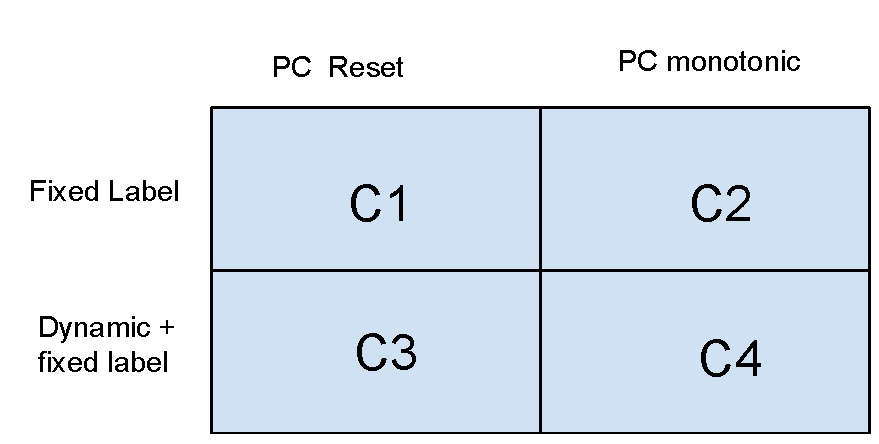
\includegraphics[width=0.6\textwidth]{category}
		\centering
		\caption{Category of constraint generator}
		\label{fig:set}
	\end{figure*}
	\begin{figure*}[h]
		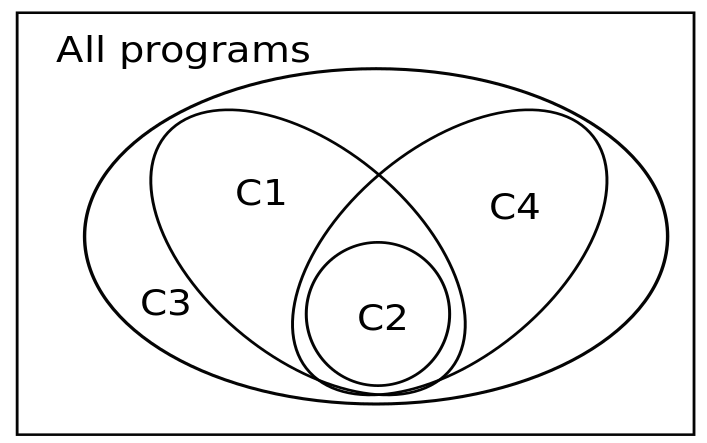
\includegraphics[width=0.6\textwidth]{rsz_set}
		\centering
		\caption{Set diagram}
		\label{fig:set}
	\end{figure*}
	Figure \ref{fig:set} shows the relationship between set of programs declared secure by all constraint generator. C1-C4 are abbreviation for category 1 - category 4. Number of constraints is inversely proportional to size of set of program declared secure, because more constraints means high probability of violation of security. In category 1 generator generates many false constraints because of absence of dynamic label, but category 3 uses dynamic labels with fixed so it reduces number of constraints. Constraints generated by category 1 are superset of constraints generated by category 3 this relationship shows that set of program declared secure by C1 must be subset of C3. Similarly C2 and C4 differ by use of dynamic labels so set of accepted program by C2 is a subset of set of programs accepted by C4. Use of monotonic PC label helps to capture global information flows so use of monotonic PC label increases the number of constraints. C3 and C4 differ by use of PC label scheme, C4 using monotonic PC and C3 using PC reset so constraints generated by C4 are superset of constraints generated by C3 so set of accepted programs of C4 must be subset of C3. Similarly C2 and C1 differ by PC label scheme so set of accepted programs is a subset of set of programs accepted by C1.    
	\begin{figure}
		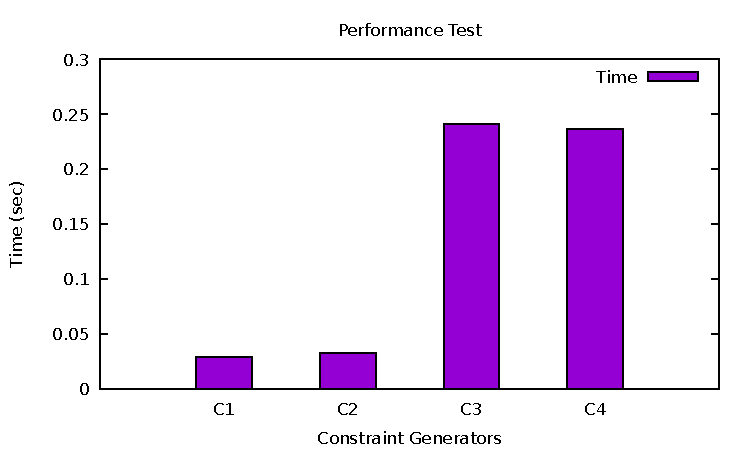
\includegraphics[width=1\textwidth]{graph.pdf}
		\centering
		\caption{Performance test}
		\label{fig:ptest}
	\end{figure}
	\pagebreak
	Figure \ref{fig:ptest} shows the average time taken in processing one copy program by all four generator. 
	Time taken in order C1 < C2 < C4 < C3. C4 taking little less time than C3 because of optimization in label generation, this optimization uses property of monotonic PC so it can not applied in C3.
\chapter{Constraint Verification with RWFM Labels}
\label{ch:label}
Information flow policies require some data related to objects and subjects to enforce any security protocol on them.
Each object and subject needs to specify information related to permission like who can read, who can write etc. Label or security class is a way to represent this information. Information flow policies add some prerequisite condition with each operation on objects based on labels of objects and subject.
\section{RWFM label \cite{rwfm}}
Reader Writer Flow Model label has three tuple (s,R,W)
the first s is a subject, R is a set of subjects allowed to read object, W is a set of subjects allowed to write and subjects who influenced this object so far. 
\subsection{Secure Information Flow}
All information flow security models follow property of lattice because, for secure flow, information must flow from less secure class or label to more secure class or label, any reverse flow is a violation of security.
So each information flow model redefines $\leqslant$ operator to check validity of flow.\\
\textbf{Label1} = ($s_1,R_1,W_2$), \textbf{Label2} = ($s_2,R_2,W_2$)\\
information can flow from Label1 to Label2 if and only if $R_1 \supseteq R_2$ and $W_1 \subseteq W_2$.  
\subsection{Definition of Join and Meet operations \cite{rwfm}}
\textbf{Join:} Label1 $\oplus$ Label2 = $(s_3,R_1 \cap R_2, W_1 \cup W_2)$\\
\hspace*{0.6cm}\textbf{Meet:} Label1 $\otimes$ Label2 = $(s_3,R_1 \cup R_2, W_1 \cap W_2)$
\subsection{Create, Read and Write operations on objects with RWFM label \cite{rwfm}}
If a subject $s^{(s,R_1,W_1)}$ creates object o, o will be assigned a default label derived from subject is $(s,R_1,W_1 \cup \{s\})$.
Clearance of subject s is assumed (s,$R_s$,$W_s$), clearance is used to set an upper bound on labels of a subject.\\
\textbf{Read:} A subject $s^{(s_1,R_1,W_1)}$ can read object $o^{(s_2,R_2,W_2)}$ if and only if s $\in$ $R_2$ and ($R_1$ $\cap$ $R_2$) $\supseteq$ $R_s$ $\land$ ($W_1$ $\cup$ $W_2$) $\subseteq$ $W_s$. after read operation label of subject s changes into $(s_1,R_1 \cap R_2, W_1 \cup W_2)$\\
 \textbf{Write:} A subject $s^{(s_1,R_1,W_1)}$ can read object $o^{(s_2,R_2,W_2)}$ if and only if s $\in$ $W_2$ and $R_1 \supseteq R_2 \land W_1 \subseteq$ W2. 
\section{Constraint Verification}
First of all constraint checker script processes inputs and populate data structures. Inputs are two files, one has all constraints generated by our constraint generator script, other has labels of each object provided by user. Figure \ref{fig:script2} shows modules of script2 with flow of control. After preprocessing of given constraints and labels, script provides answer to following queries.\\ 
\begin{figure*}[ht]
	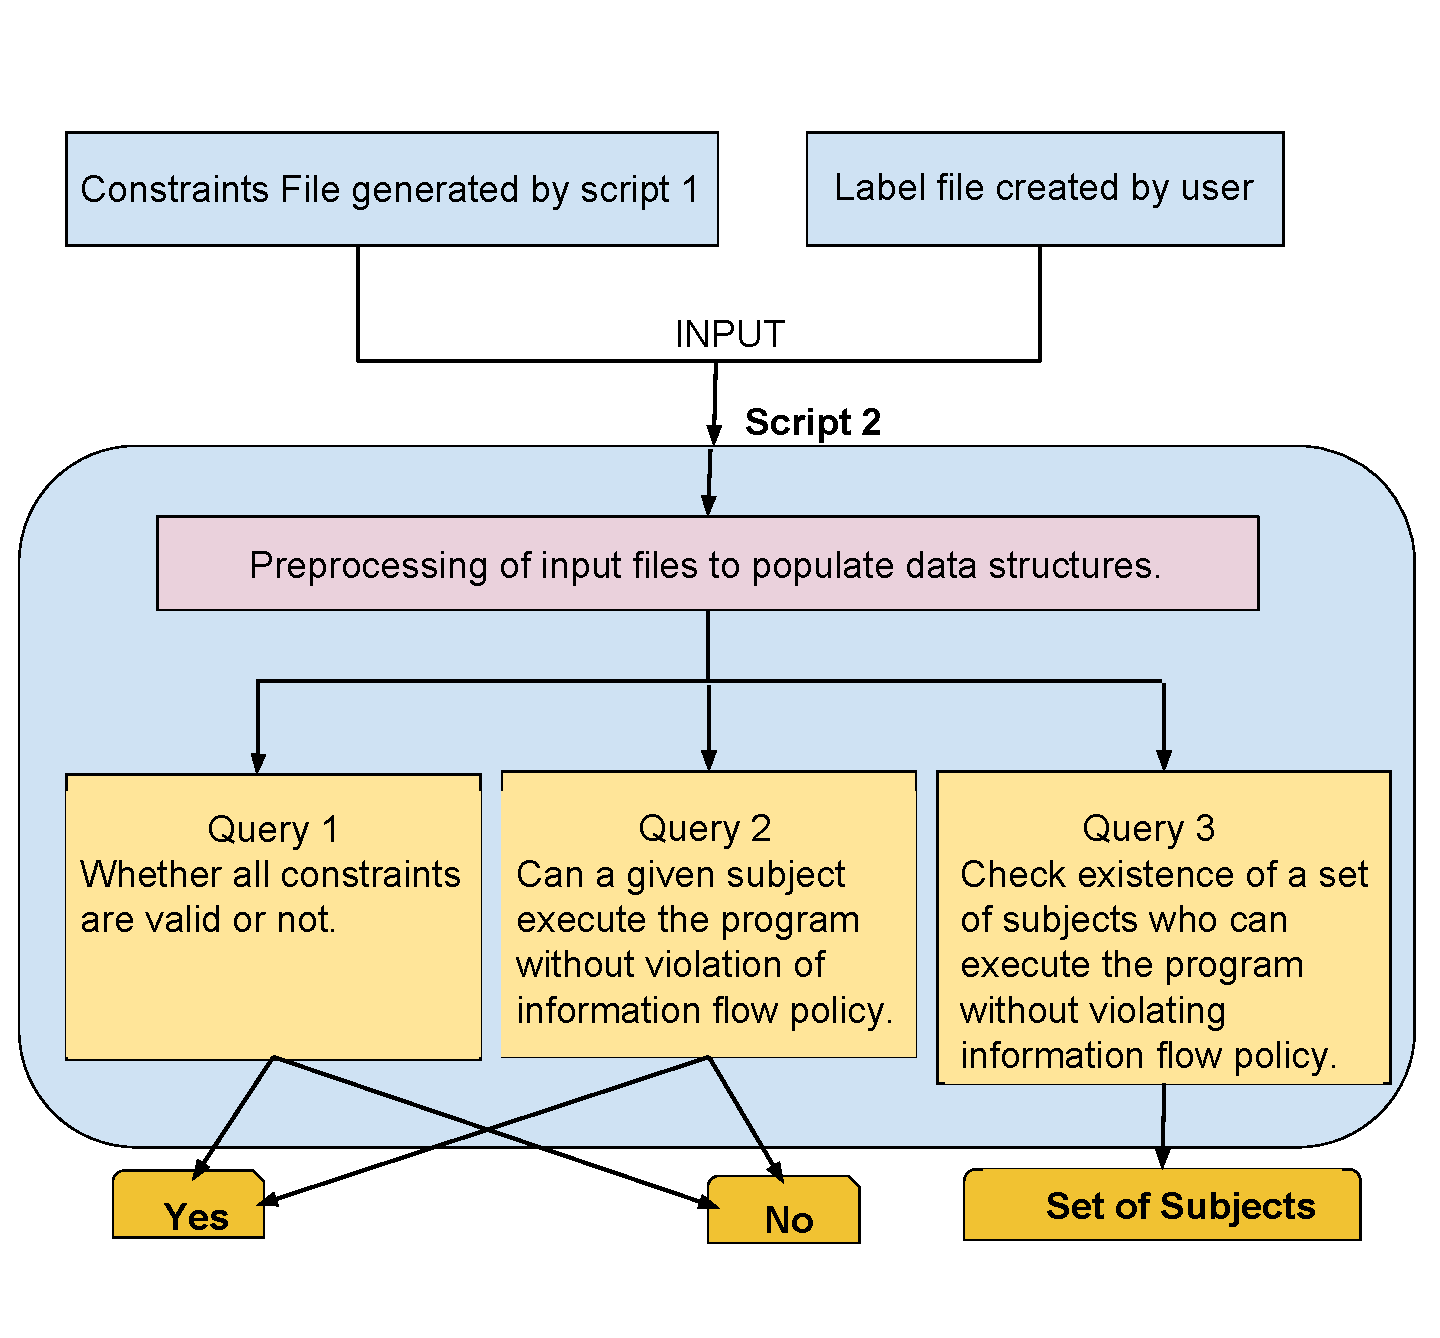
\includegraphics[width=0.7\textwidth]{constraint_checker.pdf}
	\centering
	\caption{Block diagram of script2}
	\label{fig:script2}
\end{figure*}
\begin{enumerate}
	\item{\textbf{Whether all constraints are valid or not.}\\
		Constraint format in input file : \dud{x} $\le$ \dud {y}.\\
		Format of RWFM labels : label(x) ($s_1,R_1,W_1$)\\
		\hspace*{4.5cm}label(y) ($s_2,R_2,W_2$)\\
		Definition of $\leqslant_{RWFM}$ operator in RWFM model  : label(x) $\leqslant_{RWFM}$ label(y) if only if $R_1 \supseteq R_2$ and $ W_1 \subseteq W_2 $ \hspace*{1cm}\cite{rwfm}\\
		Script reads all constraints from input file one by one then converts all objects involved in constraint into RWFM label and  checks whether they follow $\leqslant_{RWFM}$, if any constraint fails to follow $\leqslant_{RWFM}$ then returns false otherwise true.
		} 
	\item{\textbf{Can a given subject execute the program without violation of information flow policy.}\\
		\begin{figure*}
			\centering
			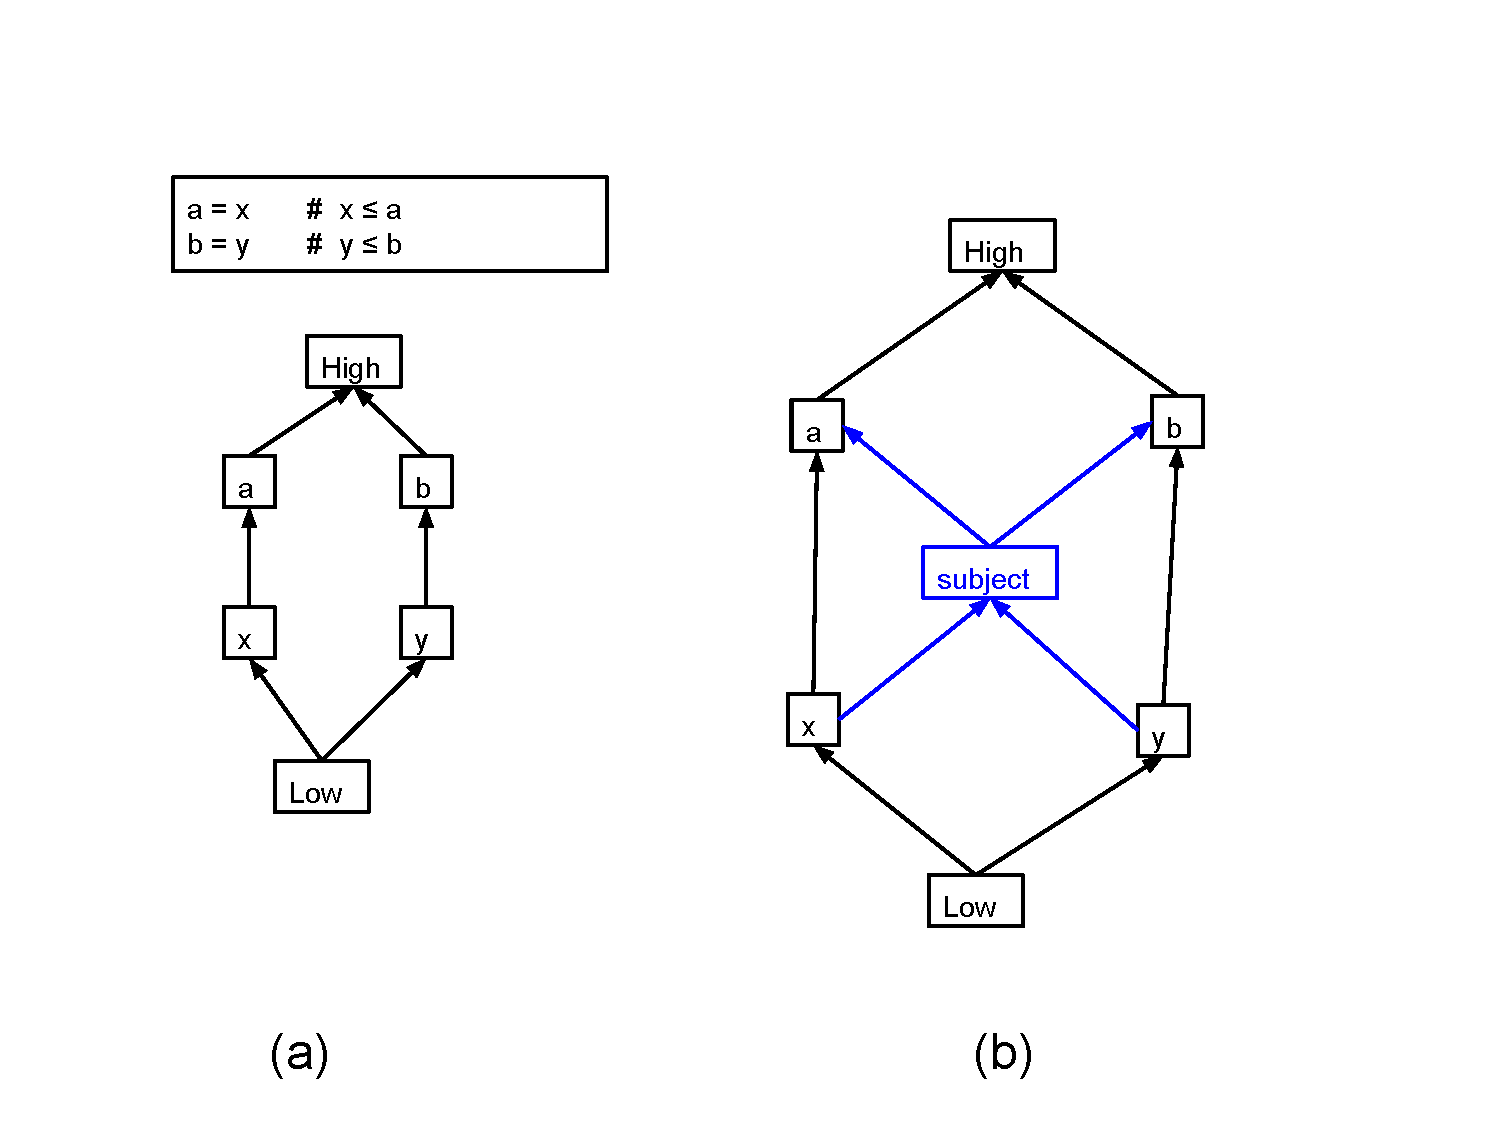
\includegraphics[width=0.8\textwidth]{sub}
			\caption{Lattice for information flow in a =x and y =b,(a)without subject (b) with subject.}
			\label{fig:sublattice}
		\end{figure*}
		In the previous case, we are checking constraints without considering the subject, but now a subject is given as input and we have to check whether given subject has all required permissions to execute all statements without violation of information flow policy. Figure \ref{fig:sublattice} shows that subject needs to read x and write a in order to execute a = x, so it must follow label(x)  $\leqslant_{RWFM}$ label(subject) and label(subject) $\leqslant_{RWFM}$ label(a) to maintain secure information flow. If the subject does not have required permissions for any statement then script returns false otherwise true.     
		}
    \item{\textbf{Check existence of a set of subjects who can execute the program without violating information flow policy. }\\
    	In this case, we need to find a maximal set of those subjects who can pass 2nd case. A naive way to implement it: for each subject run the 2nd test and if it passes, add it in a set; after checking all subjects this set will be desired output. There is an efficient way to do it, any subject can pass 2nd test if and only if it is present in reader set of all objects which lie on the left side of $\leqslant$ operator in constraints and it is  present in writer set of all objects which lie on the right side of $\leqslant$ operator in constraints . So we take the stepwise intersection of all reader sets of objects tht lie in left side of $\leqslant$ operator in constraints and writer sets of all objects that lie on the right side of $\leqslant$ operator in constraints.\\ \textbf{Example:} constraint is given in equation \ref{eqn:cons}\\
    	Conversion of security class of objects into RWFM labels: $x^{(s,R_1,W_1)}$, $y^{(s,R_2,W_2)}$, $z^{(s,R_3,W_3)}$.\\
    	Output of script: $R_1 \cap R_2 \cap W_3$
    	 \begin{equation}\label{eqn:cons}
    	 \dud{x} \oplus \dud{y} \leqslant \dud{z}
    	 \end{equation}
    	       
    }	
\end{enumerate}
%\section{Comparision between Syntatic labels and RWFM label}
%\textbf{Syntatic label(Security class)} : Denning's book \cite{denning} described the use of security class for a multi-level security system in chapter 5, where security class is a pair of two fields (A,C), A: authority label and C: category.     


\chapter{Conclusion \& Future work}
\label{ch:conclusion}
We have implemented various algorithms for constraint generation for capturing information flow in program, category 4 algorithm represents intuitive notion of correct security. Second part is verification of constraints using RWFM \cite{rwfm} is also implemented. We considered the subject in information flow analysis, it helps to deal with real world problems related with information flow.\\
\textbf{Future work}
\begin{itemize}
	\item Information flow analysis on python data structures list, dictionary etc.
	\item Information flow analysis related to dynamic types and objects in python
	\item Implementation for all features of python.  
\end{itemize} 


\chapter{Python Syntax}
\label{ch:thread}
\begin{enumerate}
\item if e == 1 then x = y else x = z : \\
\begin{lstlisting}[ numbers=left, mathescape,%
caption={if else, indentation is must}]
if e == 1:
	x = y
else:
	x = z 
\end{lstlisting} 

\item while( x < y ) \{ x = y; z += 1 \} 
\begin{lstlisting}[ mathescape,%
caption={while loop}]
while x < y:
	x = y
	z += 1
\end{lstlisting}
\item \textbf{function}: (x is a global variable) foo(int z, int y) { x+=1;int y; y=1; return y; }
\begin{lstlisting}[language=Python, caption=threads]
def foo(z , y):
	global x
	x +=1
	y = 1
	return y
\end{lstlisting}

\item threads
\begin{lstlisting}[language=Python, caption=threads]
import thread
import time
import threading

s0 = threading.Event()

def thread1():
	global x
	s0.set()
	s0.clear()
	s0.wait()

thread.start_new_thread(thread1,())
\end{lstlisting}

\end{enumerate}
\begin{appendices}
	\chapter{Python Script category 1: Constraint Generator}
	\label{ch:p1}
	\lstinputlisting[language=Python]{p1.py}
	\chapter{Python Script category 2: Constraint Generator}
	\label{ch:p2}
	\lstinputlisting[language=Python]{p2.py}
	\chapter{Python Script category 3: Constraint Generator}
	\label{ch:p3}
	\lstinputlisting[language=Python]{p3.py}
	\chapter{Python Script category 4: Constraint Generator}
	\label{ch:p4}
	\lstinputlisting[language=Python]{p4.py}
	\chapter{Python Script 2: Constraint Checker}
	\label{ch:script2}
	\lstinputlisting[language=Python]{constraint_checker.py}
	\chapter{Copy Programs}
	\label{ch:programs}
	\lstinputlisting[language=Python]{programs.py}
	
\end{appendices}


%\addcontentsline{toc}{chapter}{References}
\bibliography{mylit}
%\bibliographystyle{unsrt}

\end{document}